\documentclass[12pt,a4paper]{article}

% ─── Page Layout ───────────────────────────────────────────────────────────────
\usepackage[a4paper, margin=0.8in, headheight=14pt]{geometry}

% ─── Fonts (XeLaTeX) ───────────────────────────────────────────────────────────
\usepackage{fontspec}
\usepackage{unicode-math}
\setmainfont{TeX Gyre Pagella}
\setmonofont[Scale=0.88]{TeX Gyre Cursor}
\setmathfont{Latin Modern Math}

% ─── Packages ──────────────────────────────────────────────────────────────────
\usepackage{xcolor}
\usepackage{colortbl}
\usepackage{titlesec}
\usepackage{enumitem}
\usepackage{tabularx}
\usepackage{booktabs}
\usepackage{array}
\usepackage{amsmath}
\usepackage{tikz}
\usetikzlibrary{shapes.geometric, arrows.meta, positioning, calc, fit, decorations.pathreplacing, patterns, backgrounds}
\usepackage{tcolorbox}
\tcbuselibrary{skins, breakable}
\usepackage{hyperref}
\usepackage{fancyhdr}
\usepackage{graphicx}
\usepackage{microtype}
\hyphenpenalty=10000
\exhyphenpenalty=10000
\sloppy
\usepackage{caption}
\usepackage{setspace}
\usepackage{multirow}
\usepackage{tocloft}

% ─── Q&A helper ────────────────────────────────────────────────────────────────
\newcommand{\Q}[1]{\textbf{#1}\par\noindent\ignorespaces}

% ─── Colour Palette ────────────────────────────────────────────────────────────
\definecolor{myred}{RGB}{196,30,58}
\definecolor{mydark}{RGB}{30,30,50}
\definecolor{mygreen}{RGB}{14,120,80}
\definecolor{myteal}{RGB}{0,130,140}
\definecolor{myamber}{RGB}{180,100,0}
\definecolor{mypurple}{RGB}{100,30,160}
\definecolor{mygray}{RGB}{246,247,249}
\definecolor{mgframe}{RGB}{180,185,200}
\definecolor{watermark}{RGB}{145,150,170}
\definecolor{hdrred}{RGB}{250,232,235}
\definecolor{hdrgreen}{RGB}{220,244,233}
\definecolor{hdrteal}{RGB}{220,242,244}
\definecolor{hdramber}{RGB}{253,242,215}
\definecolor{hdrpurple}{RGB}{238,228,255}
\definecolor{hdrgray}{RGB}{238,240,245}
\definecolor{rowalt}{RGB}{250,251,253}

% ─── Section Formatting ────────────────────────────────────────────────────────
\titleformat{\section}{\large\bfseries\color{myred}}{\thesection.}{0.5em}{}[\vspace{1pt}{\color{myred}\rule{\linewidth}{0.8pt}}]
\titleformat{\subsection}{\normalsize\bfseries\color{myteal}}{\thesubsection}{0.5em}{}
\titlespacing*{\section}{0pt}{18pt}{7pt}
\titlespacing*{\subsection}{0pt}{11pt}{4pt}

% ─── Paragraph ─────────────────────────────────────────────────────────────────
\setlength{\parindent}{0pt}
\setlength{\parskip}{4pt}

% ─── TOC Styling ───────────────────────────────────────────────────────────────
\renewcommand{\cfttoctitlefont}{\large\bfseries\color{myred}}
\renewcommand{\cftaftertoctitle}{\par\noindent{\color{myred}\rule{\linewidth}{0.8pt}}}
\setlength{\cftbeforetoctitleskip}{0pt}
\setlength{\cftaftertoctitleskip}{6pt}
\renewcommand{\cftsecfont}{\normalsize\bfseries\color{mydark}}
\renewcommand{\cftsecpagefont}{\normalsize\bfseries\color{mydark}}
\renewcommand{\cftsecleader}{\cftdotfill{\cftdotsep}}
\setlength{\cftbeforesecskip}{7pt}
\renewcommand{\cftsubsecfont}{\small\color{mydark}}
\renewcommand{\cftsubsecpagefont}{\small\color{mydark}}
\setlength{\cftbeforesubsecskip}{3pt}
\setlength{\cftsubsecindent}{1.4em}

% ─── Table helpers ─────────────────────────────────────────────────────────────
\renewcommand{\arraystretch}{1.45}
\setlength{\tabcolsep}{6pt}
\arrayrulecolor{mydark}
\newcolumntype{B}[1]{>{\small\bfseries\raggedright\arraybackslash}m{#1}}
\newcolumntype{Y}{>{\small\raggedright\arraybackslash}X}
\renewcommand{\tabularxcolumn}[1]{m{#1}}

% ─── Header / Footer ───────────────────────────────────────────────────────────
\pagestyle{fancy}
\fancyhf{}
\fancyhead[L]{\small\color{myred}\textbf{OE-EC804A}\;\color{mydark}--- Artificial Intelligence}
\fancyhead[R]{\small\color{myteal}\textbf{Module 3 Notes}}
\fancyfoot[C]{\small\color{mydark}\thepage}
\fancyfoot[R]{\small\color{watermark}\textit{\copyright\ Biraj Sarkar}}
\renewcommand{\headrulewidth}{0.5pt}
\renewcommand{\footrulewidth}{0.3pt}

% ─── Hyperref ──────────────────────────────────────────────────────────────────
\hypersetup{colorlinks=true, linkcolor=myteal, urlcolor=myteal,
  pdfauthor={Biraj Sarkar}, pdftitle={OE-EC804A --- Module 3 Notes}}

% ─── tcolorbox styles ──────────────────────────────────────────────────────────
\tcbset{
  tikzbox/.style={colback=mygray, colframe=mgframe, boxrule=0.6pt, arc=4pt,
    left=8pt, right=8pt, top=6pt, bottom=6pt,
    colbacktitle=mgframe, coltitle=mydark, fonttitle=\small\bfseries, unbreakable},
  defbox/.style={colback=hdrgreen, colframe=mygreen, boxrule=0.8pt, arc=4pt,
    left=9pt, right=9pt, top=6pt, bottom=6pt,
    colbacktitle=mygreen, coltitle=white, fonttitle=\small\bfseries},
  formulabox/.style={colback=hdrteal, colframe=myteal, boxrule=0.8pt, arc=4pt,
    left=9pt, right=9pt, top=7pt, bottom=7pt,
    colbacktitle=myteal, coltitle=white, fonttitle=\small\bfseries},
  examplebox/.style={colback=hdramber, colframe=myamber, boxrule=0.8pt, arc=4pt,
    left=9pt, right=9pt, top=6pt, bottom=6pt,
    colbacktitle=myamber, coltitle=white, fonttitle=\small\bfseries},
  masonbox/.style={colback=hdrpurple, colframe=mypurple, boxrule=0.8pt, arc=4pt,
    left=9pt, right=9pt, top=6pt, bottom=6pt,
    colbacktitle=mypurple, coltitle=white, fonttitle=\small\bfseries},
  exambox/.style={colback=hdrpurple, colframe=mypurple, boxrule=1pt, arc=5pt,
    left=10pt, right=10pt, top=8pt, bottom=8pt,
    colbacktitle=mypurple, coltitle=white, fonttitle=\bfseries,
    breakable, title after break={\textbf{Frequently Asked / Viva Questions (contd.)}}}
}
\tcbset{breakable}

% ─── TikZ styles ───────────────────────────────────────────────────────────────
\tikzset{
  block/.style={rectangle, draw=myteal, fill=hdrteal, text width=2.2cm, align=center, minimum height=0.9cm, font=\small, rounded corners=3pt},
  cnode/.style={circle, draw=mypurple, fill=hdrpurple, minimum size=0.9cm, font=\small\bfseries},
  arrow/.style={-Stealth, thick, color=mydark},
  line/.style={thick, color=mydark}
}

\begin{document}

% ═══════════════════════════════════════════════════════════════════════════════
% TITLE BLOCK
% ═══════════════════════════════════════════════════════════════════════════════
\begin{center}
  \hfill \textit{Exam-Ready Short Notes} \\
  \vspace{6pt}
  {\LARGE\bfseries\color{myred} OE-EC804A --- Artificial Intelligence}\\[5pt]
  {\normalsize\color{mydark} Semester VIII \quad$\bullet$\quad 3L:0T:0P \quad$\bullet$\quad 3 Credits}\\[3pt]
  {\normalsize\color{myteal}\textbf{Module 3: Informed Search \& Constraint Satisfaction Problems}}\\[3pt]
  {\small\color{mydark} CGEC \;$|$\; B.Tech ECE (2023--27) \;$|$\; \textit{Biraj Sarkar}}
\end{center}
\vspace{2pt}
\noindent{\color{myred}\rule{\linewidth}{1.5pt}}
\vspace{2pt}

\hypersetup{linkcolor=mydark}
\tableofcontents
\hypersetup{linkcolor=myteal}
\newpage

% ===============================================================================
\section{Informed (Heuristic) Search Strategies}
% ===============================================================================

Informed search strategies use domain-specific knowledge provided by a \textbf{Heuristic Function} $h(n)$ to guide the search towards goal states more efficiently.

\begin{tcolorbox}[defbox, title={Definition of a Heuristic Function}]
  A \textbf{Heuristic Function} $h(n)$ estimates the cost of the cheapest path from state $n$ to a goal state. For any goal state $g$, $h(g) = 0$.
\end{tcolorbox}

\subsection{1. Greedy Best-First Search}
\begin{itemize}[leftmargin=*, itemsep=3pt]
  \item \textbf{Evaluation Function:} $f(n) = h(n)$.
  \item Expands the node that appears to be closest to the goal.
  \item \textbf{Properties:} Incomplete in looped graphs; non-optimal. Time and Space complexity $O(b^m)$ worst-case.
\end{itemize}

\subsection{2. A* Search Algorithm}
A* combines the cost-so-far $g(n)$ and estimated remaining cost $h(n)$.

\begin{tcolorbox}[formulabox, title={A* Evaluation Function}]
  \begin{equation}
    f(n) = g(n) + h(n)
  \end{equation}
  where:
  \begin{itemize}[leftmargin=*, noitemsep]
    \item $g(n)$: Exact path cost from initial state to node $n$.
    \item $h(n)$: Estimated cost from node $n$ to goal state.
    \item $f(n)$: Estimated total cost of path through $n$ to goal.
  \end{itemize}
\end{tcolorbox}

\subsection{Conditions for A* Optimality}
\begin{enumerate}[leftmargin=*, itemsep=4pt]
  \item \textbf{Admissibility (Tree Search Optimality):}
    A heuristic $h(n)$ is admissible if it \textbf{never overestimates} the true cost to reach the goal:
    \begin{equation}
      h(n) \le h^*(n) \quad \forall n
    \end{equation}
    where $h^*(n)$ is the true minimum cost from $n$ to goal.
  
  \item \textbf{Monotonicity / Consistency (Graph Search Optimality):}
    A heuristic $h(n)$ is consistent if for every node $n$ and successor $n'$ generated by action $a$:
    \begin{equation}
      h(n) \le c(n, a, n') + h(n')
    \end{equation}
    This satisfies the triangle inequality and guarantees $f(n)$ is non-decreasing along any path.
\end{enumerate}

\subsection{On-line Search Agents and Unknown Environments}
Unlike offline search algorithms (which compute a complete solution path before taking their first action), an \textbf{On-line Search Agent} interleaves computation and action: it acts, observes the new state, and decides its next move.

\begin{tcolorbox}[defbox, title={On-line Search Agent}]
  An \textbf{On-line Search Agent} operates in unknown or dynamic environments by exploring state space physically. It computes an action, executes it in the environment, senses the resulting state $s'$, and updates its internal map.
\end{tcolorbox}

\begin{itemize}[leftmargin=*, itemsep=3pt]
  \item \textbf{Offline vs. On-line Search:} Offline agents compute the full path in a simulator before moving. On-line agents move in the physical world to discover state transitions and costs.
  \item \textbf{Competitive Ratio:} Evaluates on-line search performance by comparing actual path cost incurred to the optimal path cost if the environment were known in advance.
  \item \textbf{LRTA* (Learning Real-Time A*):} An on-line search algorithm that updates heuristic estimates $H(s)$ of visited states based on neighbor cost:
    \begin{equation}
      H(s) \leftarrow \min_{a \in Actions(s)} \left[ c(s, a, s') + H(s') \right]
    \end{equation}
\end{itemize}

% ===============================================================================
\section{Constraint Satisfaction Problems (CSPs)}
% ===============================================================================

\begin{tcolorbox}[defbox, title={Definition of a CSP}]
  A \textbf{Constraint Satisfaction Problem (CSP)} is defined by a triple $(X, D, C)$:
  \begin{itemize}[leftmargin=*, noitemsep]
    \item $X = \{X_1, X_2, \dots, X_n\}$: Set of variables.
    \item $D = \{D_1, D_2, \dots, D_n\}$: Set of domains (possible values for each variable).
    \item $C = \{C_1, C_2, \dots, C_m\}$: Set of constraints specifying allowable value combinations.
  \end{itemize}
\end{tcolorbox}

\begin{tcolorbox}[tikzbox, title={Constraint Graph Representation (Map Coloring Example)}]
\centering
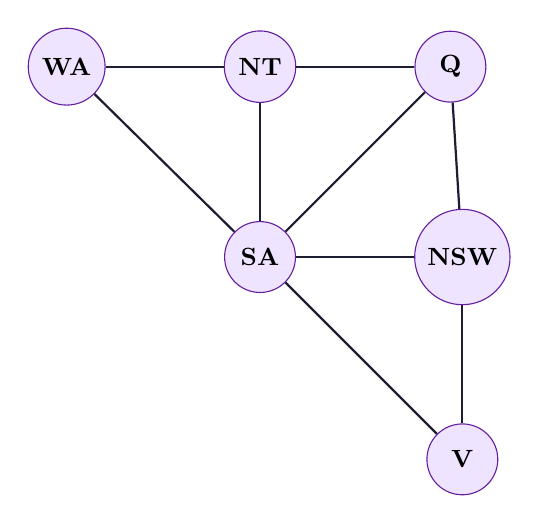
\begin{tikzpicture}[node distance=1.5cm, auto]
  \node [cnode] (wa) {WA};
  \node [cnode, right=of wa] (nt) {NT};
  \node [cnode, right=of nt] (q) {Q};
  \node [cnode, below=of nt] (sa) {SA};
  \node [cnode, right=of sa] (nsw) {NSW};
  \node [cnode, below=of nsw] (v) {V};

  \draw [line] (wa) -- (nt);
  \draw [line] (wa) -- (sa);
  \draw [line] (nt) -- (sa);
  \draw [line] (nt) -- (q);
  \draw [line] (q) -- (sa);
  \draw [line] (q) -- (nsw);
  \draw [line] (sa) -- (nsw);
  \draw [line] (sa) -- (v);
  \draw [line] (nsw) -- (v);
\end{tikzpicture}
\end{tcolorbox}

\subsection{Backtracking Search for CSPs}
Backtracking search is a depth-first search that chooses values for one variable at a time and backtracks when a variable has no legal values left.

\begin{tcolorbox}[examplebox, title={Heuristics for CSP Backtracking}]
  \begin{enumerate}[leftmargin=*, noitemsep]
    \item \textbf{Minimum Remaining Values (MRV):} Choose variable with fewest legal values remaining ("fail-first" heuristic).
    \item \textbf{Degree Heuristic:} Choose variable involved in largest number of constraints on unassigned variables.
    \item \textbf{Least Constraining Value (LCV):} Choose value that rules out fewest choices for neighboring variables.
  \end{enumerate}
\end{tcolorbox}

\subsection{Constraint Propagation \& AC-3 Algorithm}
Constraint propagation enforces local consistency to prune search spaces early.

\begin{itemize}[leftmargin=*, itemsep=3pt]
  \item \textbf{Forward Checking:} When variable $X$ is assigned, remove inconsistent values from domains of unassigned neighbors.
  \item \textbf{Arc Consistency (AC-3):} Arc $X_i \to X_j$ is consistent if for every value $x \in D_i$, there exists an allowed value $y \in D_j$.
\end{itemize}

\subsection{Local Search for CSPs (Min-Conflicts Algorithm)}
Unlike backtracking search which operates on partial assignments, local search algorithms for CSPs use a \textbf{complete-state formulation}: every variable is initially assigned a value (even if constraints are violated).

\begin{tcolorbox}[defbox, title={Min-Conflicts Heuristic}]
  In each iteration, \textbf{Min-Conflicts} randomly selects a conflicted variable $X_i$ and reassigns it the value $v \in D_i$ that minimizes the total number of constraint violations across the CSP.
\end{tcolorbox}

\begin{itemize}[leftmargin=*, itemsep=3pt]
  \item \textbf{Algorithm Mechanism:} Start with a complete assignment $\to$ pick a conflicted variable $X$ at random $\to$ set $X$ to value minimizing constraint violations $\to$ repeat until solution or step limit.
  \item \textbf{Performance:} Solves $N$-Queens for $N = 1,000,000$ in seconds; space complexity is $O(n)$ (linear).
  \item \textbf{Escaping Local Minima:} Uses random walks, simulated annealing, or random restarts to escape plateau states.
\end{itemize}

\newpage
\begin{center}
  {\large\bfseries\color{myred} Quick Revision --- Module 3}\\[3pt]
  {\small\color{mydark} Informed Search \& Constraint Satisfaction Problems $|$ OE-EC804A}
\end{center}
\noindent{\color{myred}\rule{\linewidth}{1.2pt}}
\vspace{4pt}

\begin{tcolorbox}[formulabox, title={\textbf{Key Concepts and Metrics at a Glance}}]
\renewcommand{\arraystretch}{1.35}
\begin{tabularx}{\linewidth}{B{4.5cm} X}
A* Evaluation Function & $f(n) = g(n) + h(n)$ \quad ($g(n)$ cost-so-far, $h(n)$ estimated remaining cost) \\[4pt]
Admissibility Condition & $h(n) \le h^*(n)$ \quad (Heuristic never overestimates true cost to goal) \\[4pt]
Consistency Condition & $h(n) \le c(n, a, n') + h(n')$ \quad (Satisfies triangle inequality along edges) \\[4pt]
CSP Formalization & Triple $(X, D, C)$ of Variables, Domains, and Constraints \\[4pt]
Min-Conflicts Heuristic & Local search reassigning conflicted variable value to minimize violations. \\
\end{tabularx}
\end{tcolorbox}

\begin{tcolorbox}[defbox, title={\textbf{One-Line Definitions}}]
  \begin{itemize}[leftmargin=*, noitemsep]
    \item \textbf{Admissible Heuristic:} A heuristic that never overestimates the actual cost to reach goal.
    \item \textbf{Consistent Heuristic:} A heuristic obeying triangle inequality along graph edges.
    \item \textbf{Arc Consistency (AC-3):} State where every value in a variable domain has a valid partner in neighbor domains.
    \item \textbf{MRV Heuristic:} Chooses the variable with the fewest remaining legal domain choices.
  \end{itemize}
\end{tcolorbox}

\begin{tcolorbox}[exambox, title={\textbf{Frequently Asked / Viva Questions}}]
  \begin{enumerate}[topsep=0pt, label=\textbf{Q\arabic*.}, itemsep=5pt]
    \item \Q{Define A* search. What is its evaluation function?}
    A* evaluates nodes using $f(n) = g(n) + h(n)$, combining cost-so-far $g(n)$ and heuristic estimate $h(n)$.

    \item \Q{What is an Admissible Heuristic?}
    A heuristic $h(n)$ that never overestimates true cost to goal ($h(n) \le h^*(n)$).

    \item \Q{Differentiate between Admissibility and Consistency.}
    Admissibility guarantees optimality for tree search. Consistency ($h(n) \le c(n,a,n') + h(n')$) guarantees $f(n)$ is non-decreasing, ensuring optimality for graph search without re-opening nodes.

    \item \Q{Define CSP formally.}
    A triple $(X, D, C)$ where $X$ is set of variables, $D$ set of domains, and $C$ set of constraints.

    \item \Q{Explain the MRV heuristic in CSPs.}
    Minimum Remaining Values heuristic chooses the variable with fewest valid remaining choices, aiming to fail early.

    \item \Q{What is Forward Checking?}
    In CSP search, whenever variable $X$ is assigned, any inconsistent values are pruned from neighboring unassigned variables.

    \item \Q{What is the AC-3 algorithm?}
    An algorithm that enforces arc consistency across all variable pairs in a CSP constraint graph.

    \item \Q{Compare Greedy Best-First Search and A* Search.}
    Greedy uses $f(n) = h(n)$ (fast, non-optimal). A* uses $f(n) = g(n) + h(n)$ (optimal if $h$ is admissible).

    \item \Q{What is Manhattan Distance heuristic in 8-puzzle?}
    Sum of absolute differences in horizontal and vertical coordinates of tiles from goal positions.

    \item \Q{Why is LCV used for value selection in CSPs?}
    Least Constraining Value maximizes flexibility for remaining variables, leaving maximal choices open.
  \end{enumerate}
\end{tcolorbox}

\end{document}
